\chapter{De lo simple a lo complejo}

Dentro del marco de los sistemas complejos se manejan varias ramas muy interesantes que le dan su esencia, desde los sistemas dinámicos discretos, dinámica no lineal, teoría de redes complejas, termodinámica fuera de equilibrio, modelos basados en agentes, entre otras. Cada una de ellas aporta un valioso contenido al sistema complejo que se quiera estudiar y analizar dependiendo de sus componentes. Delimitar el área de los sistemas complejos aún resulta una labor complicada debido a su gran \textit{diversidad}, sin embargo, se sabe de la existencia de ciertas características que todo sistema complejo comparte. Los sistemas complejos cuentan con entes: \textit{conectados, interdependientes, dependientes del camino, emergentes} entre otros. El presente trabajo tiene como propósito mostrar al lector cada una de estas características con el objeto de estudio que se va a proponer como piedra angular.\\
\\
Para llegar a conocer nuestra piedra angular primero será necesario delimitar las áreas que intervendrán en la discusión constante de este texto. Se ocupará un \textit{sistema dinámico no-lineal} bajo el soporte de una \textit{red compleja}. La Dinámica no lineal es la rama de los sistemas dinámicos continuos en donde el comportamiento del sistema no se rige por la suma de los comportamientos de sus descriptores. Por ejemplo, una neurona y la suma del comportamiento de las neuronas de un cerebro no puede explicar la emergencia de la consciencia. Por otro lado las redes complejas es la extensión de la \textit{teoría de grafos} aplicada a escenarios comunes de la naturaleza y de la vida cotidiana, tales como redes ecológicas, redes sociales, redes comerciales etc. Su importancia radica en las propiedades que se le pueden extraer para interpretar información sobre la estructura de la red y de la red misma.

\section{Revisión de sistemas lineales.}

En los cursos de ecuaciones diferenciales de cuarto semestre\footnote{citar a Blanchard y Devaney} es obligado abordar el tema de los sistemas de ecuaciones diferenciales lineales con el objetivo de explorar en un primer nivel el comportamiento de diversas cantidades que interactúan y evolucionan en el tiempo. Las ecuaciones diferenciales son la herramienta para modelar fenómenos y su evolución en el tiempo; nos permite trazar soluciones que describen su trayectoria. Dicho de otra forma, son la herramienta para anticipar el comportamiento del fenómeno aunque en la vida real no es tan simple como suena.
\begin{definición}
	Un sistema de ecuaciones diferenciales lineales es una colección de $n$ ecuaciones diferenciales interrelacionadas de la forma
	\begin{equation}\label{eqn:sistemaLineal}
		\begin{split}
			\dot{x}_1 &= f_1(x_1(t),...,x_n(t))\\
			\dot{x}_2 &= f_2(x_1(t),...,x_n(t))\\
			\vdots\\
			\dot{x}_n &= f_n(x_1(t),...,x_n(t))
		\end{split}
	\end{equation}
	donde $f:\mathbb{R}^n\to\mathbb{R}$ lineal, continua y diferenciable. No esta demás recordar que para que una función se considerada lineal debe de cumplir para cualesquiera dos vectores $u,v \in\mathbb{R}^n$ y para todo $k\in\mathbb{R}$ satisface:
	\begin{itemize}
		\item [1.] $f(u+v)=f(u)+f(v)$
		\item [2.] $f(ku)=kf(u)$
	\end{itemize}
	A este cumplimiento se le conoce como \textit{principio de superposición} y el concepto se extiende cuando contamos con las soluciones del sistema lineal.
\end{definición}
Al tratarse de un sistema lineal, resulta bastante oportuno expresarlo en términos de notación matricial, es decir, una multiplicación de una matriz cuadrada $M\in\mathcal{M}_n(\mathbb{R})$ por un vector columna que tiene a todas las funciones $x_i(t)$ lineales.
\begin{align*}
	\begin{split}
			\dot{x}_1 &= a_{11}x_1(t)+\cdots+a_{1n}x_n(t)             \\
			\vdots &\qquad \vdots\qquad\qquad\vdots\qquad\quad\vdots  \\
			\dot{x}_n &= a_{n1}x_1(t)+\cdots+a_{nn}x_n(t)             
	\end{split}	          
	\qquad\ \ \, \Longleftrightarrow
	\begin{split}
		\underbrace{\begin{pmatrix}
				\dot{x}_1\\
				\vdots\\
				\dot{x}_n
		\end{pmatrix}}_{\dot{X}(t)}=\underbrace{\begin{pmatrix}
				a_{11} & \cdots & a_{1n}\\
				\vdots & \ddots & \vdots\\
				a_{n1} & \cdots & a_{nn}
		\end{pmatrix}}_{M}\underbrace{\begin{pmatrix}
		x_1(t)\\
		\vdots\\
		x_n(t)
	\end{pmatrix}}_{X(t)}
	\end{split} 
\end{align*}
en este caso las constantes de la matriz $a_{ij}\in M$ son parámetros que describen ciertas interacciones con respecto de las cantidades que intervienen en el sistema (\ref{eqn:sistemaLineal}); estas interacciones son las responsables de la dinámica del sistema, es decir, de la manera en que evoluciona en el tiempo dependiendo de sus condiciones iniciales. Es conveniente poder contar con la matriz de coeficientes ya que por si sola nos servirá para darle solución al sistema lineal y para poder conocer la estabilidad del mismo, aún sin saber la solución general. Para ahondar en el tema de la estabilidad es necesario conocer los \textit{puntos fijos} del sistema.


%%%%%%%%%%%%%%%%%%CHECHPOINT


\subsection{Puntos fijos y estabilidad del sistema.}

También llamados puntos de equilibrio son aquellos en donde las soluciones de (\ref{eqn:sistemaLineal}) permanecen constantes en el tiempo y dependiendo de su naturaleza\footnote{dictada por los elementos de la matriz de coeficientes $M$.} se establecerá si el punto y el sistema en cuestión es estable o inestable. Para poder hallarlos es necesario hacer cumplir el siguiente sistema de ecuaciones
\begin{equation*}
	\begin{split}
		\dot{x}_1 &= f_1(x_1(t),...,x_n(t))=0\\
		\dot{x}_2 &= f_2(x_1(t),...,x_n(t))=0\\
		\vdots\\
		\dot{x}_n &= f_n(x_1(t),...,x_n(t))=0
	\end{split}
	\quad\Longleftrightarrow\quad
	\begin{split}
		\begin{pmatrix}
			a_{11} & \cdots & a_{1n}\\
			\vdots & \ddots & \vdots\\
			a_{n1} & \cdots & a_{nn}
		\end{pmatrix}
		\underbrace{\begin{pmatrix}
				x_1(t)\\
				\vdots\\
				x_n(t)
		\end{pmatrix}}_{X_0}=0
	\end{split}
\end{equation*}
Para darle solución es necesario encontrar $X_0\in\mathbb{R}^n$ que lo satisfaga; en dicho caso se establece que $X_0$ es el punto fijo del sistema. Los puntos fijos son clave para entender la estabilidad de (\ref{eqn:sistemaLineal}), servirán de referencia para determinar si las soluciones tienden hacia el punto fijo o si divergen del mismo (o una combinación de ambas). Pero tan solo con determinarlo no es suficiente, para ello debemos manipular la matriz de coeficientes $M$ para saber la naturaleza de este punto fijo. Para ello necesitamos hallar los \textit{valores propios} de $M$, por tanto necesitamos determinar
\begin{equation}\label{eqn:vPropios}
	\det(M-\lambda I)=0
\end{equation}
resolviendo el polinomio característico de grado $n$ (dependiendo del tamaño del sistema), se obtendrá el conjunto de valores propios que por si mismos nos brindan demasiada información acerca de como se comportan las soluciones del sistema.

%%%%%%%%%%%%%%%%%%CHECKPOINT
\begin{proposición}\label{prp:Atractores}
	Un sistema lineal que tiene eigenvalores con parte real negativa siempre será estable, es decir, todas las soluciones tenderán hacia el punto fijo del sistema. Este punto de equilibrio del sistema con estas características es conocido como \textbf{Atractor}.
\end{proposición}
Independientemente de la elección de las condiciones iniciales, las soluciones tenderán hacia el punto fijo cuando $t\to\infty$ y se mantendrá ahí siendo resistente ante perturbaciones. Notemos que en la ec. (\ref{eqn:vPropios}) es posible tener raíces reales como complejas, dependiendo de los coeficientes de $M$. Sin embargo aunque se tengan eigenvalores complejos, la dinámica seguirá siendo la misma: se tendrán soluciones que tienden o divergen (o combinación de ambas) del punto fijo, lo que cambia es la forma en que lo hacen. Cuando las soluciones del sistema lineal divergen del punto fijo, entonces se establece que el sistema es inestable y el punto fijo asociado se le conoce como \textbf{\textit{Repulsor}}. Cualquier mínima perturbación que tenga la solución que esta ubicada en el punto fijo, hará que diverga. La combinación de los anteriores se les conoce como \textbf{\textit{Punto silla}}; se dice que es combinación porque podría acercarse al punto silla pero al hacerlo en algún momento terminará divergiendo. Es considerado también como sistema intestable ya que para $t\to\infty$ cualquier solución no trivial se irá a $\infty$.
\begin{ejemplo}\label{eg:Fuente2x2}
	Veamos un ejemplo sencillo para poder apreciar lo anterior, para ello se propone el siguiente sistema de $2\times 2$.
	$$
		\dot{X}(t)=\underbrace{\begin{pmatrix}
				2 & 2\\
				1 & 3
		\end{pmatrix}}_{M_1}X(t)
	$$
	Sacando su polinomio característico (\ref{eqn:vPropios}) tenemos los siguiente eigenvalores\footnote{para sistemas de $2\times 2$ se tiene establecido un polinomio característico que se define como $p_M(\lambda)=\lambda^2-\lambda\text{Tr}A+\det A$}
	\begin{align*}
		p_{M_1}(\lambda)&=\lambda^2-5\lambda+4 = 0\\
		\lambda_1=4 &\qquad \lambda_2=1
	\end{align*}
	Según lo que establece la Proposición \ref{prp:Atractores}, este no es un sistema que sea estable ya que sus eigenvalores tienen parte real positiva. Para poder comprobarlo necesitamos determinar la solución general del sistema asociado a $M_1$. Para ello es necesario encontrar los \textit{eigenvectores} del sistema, es decir
	\begin{align*}
		M_1\vec{v}=\lambda\vec{v}\qquad&\Longleftrightarrow\qquad (M_1-\lambda I)\vec{v}=0 \\
		\vec{v}_{\lambda_1} = \begin{bmatrix}
			1\\
			1
		\end{bmatrix}  \qquad&\qquad \vec{v}_{\lambda_2} = \begin{bmatrix}
		\frac{1}{2}\\
		-1
		\end{bmatrix}
	\end{align*}
\end{ejemplo}
\begin{teorema}\label{teo:Solgral}
	Sea $\vec{v}_0$ un eigenvector de $M$ una matriz asociada al eigenvalor $\lambda$. Entonces la función $X(t)=e^{\lambda t}\vec{v}_0$ es una solución del sistema $\vec{X}(t)=MX(t)$\footnote{ver demostración en el apéndice \ref{ch:Ap}}.
\end{teorema}
Se dice que es una solución general porque podemos seleccionar cualquier $k\in\mathbb{R}$ de tal manera que sea un múltiplo del eigenvector del sistema. En ese caso obtenemos toda una familia de soluciones posibles. Por tanto para el sistema del Ejemplo \ref{eg:Fuente2x2} se tienen las siguientes soluciones posibles:
$$X_1(t)=k_1e^{4t}\begin{bmatrix}
	1\\
	1
\end{bmatrix},\qquad\qquad X_2(t)=k_2e^{t}\begin{bmatrix}
\frac{1}{2}\\
-1
\end{bmatrix}$$
Sin embargo por tratarse de un sistema lineal, se cumple el principio de superposición lo cual significa que la solución general al sistema asociado a $M_1$ es
$$X(t)=k_1e^{4t}\vec{v}_{\lambda_1}+k_2e^{t}\vec{v}_{\lambda_2}$$
Se puede apreciar que para las soluciones separadas y la solución general del sistema asociado a $M_1$, el límite de $X(t)$ cuando $t\to\infty$ es infinito, por tanto las soluciones del Ejemplo \ref{eg:Fuente2x2} siempre van a diverger a infinito independientemente de la elección de condiciones iniciales. Cuando se trata de sistemas lineales, una solución y la suma de las soluciones siempre será solución del sistema, es decir, se pueden escribir como combinación lineal. Generalizando el concepto a un sistema de $n$ ecuaciones lineales tenemos la siguiente solución general:
\begin{equation}\label{eqn:solGral}
	X(t)=k_1e^{\lambda_1 t}\vec{v}_{\lambda_1}+k_2e^{\lambda_2 t}\vec{v}_{\lambda_2}+\cdots+k_ne^{\lambda_n t}\vec{v}_{\lambda_n}
\end{equation}
Esta solución general también aplica perfectamente para el caso en donde se tienen eigenvalores complejos, solamente que habría que descomponer mediante la relación de Euler las exponenciales, es decir, $e^{\lambda t}$ donde $\lambda=a\pm bi$ se descompone como $e^{at}\left (\cos bt+i\sin bt\right )$. Como solución se vería de la siguiente manera
\begin{equation}\label{eqn:solCompleja}
	X(t)=e^a\left (\cos bt+i\sin bt\right )\vec{v}_{\lambda}
\end{equation}
donde $\vec{v}_{\lambda}$ es un vector propio del sistema. Finalmente, en este punto tenemos todos los elementos para darle respuesta a nuestra Proposición \ref{prp:Atractores}; tanto la ecuación (\ref{eqn:solGral}) como (\ref{eqn:solCompleja}) se puede notar que si la parte real del eigenvalor del sistema es positivo, para $t\to\infty$ la exponencial también tiende a infinito y por lo tanto la solución lo hará. En contra parte, si la parte real del eigenvalor es negativa entonces la solución va a tender hacia donde los vectores propios se dirijan, particularmente hacia el punto fijo. Esto únicamente será válido si todos los eigenvalores del sistema tienen parte real negativa ya que si existe al menos uno que tenga parte real positiva eventualmente terminará divergiendo. Eso es lo que sucede con los puntos silla, quizás existan mayoría de eigenvalores con parte real negativa pero si existe al menos uno que tenga parte real positiva, eventualmente para tiempos largos la solución va a diverger. Para poder darnos una idea visual de lo que llamamos \textit{atractores}, \textit{repulsores} y \textit{puntos silla} podemos acceder al espacio fase del sistema y ver de manera integral como se comportan las soluciones del sistema lineal.

\subsection{Espacios fase}

El espacio fase es considerado como la representación geométrica de las trayectorias posibles en un sistema dinámico, en el mismo se contemplan todas las condiciones iniciales posibles y todas las trayectorias posibles que emergen de las anteriores. Aquí mismo encontramos gráficamente los puntos fijos y podemos distinguirlos cualitativamente de que naturaleza son. Las técnicas analíticas descritas anteriormente nos sirven para conocer el comportamiento sin el uso del espacio fase, pero para sistemas de $n=2,3$ podemos acceder al espacio fase y ver como son sus trayectorias. En ese sentido para sistemas con $n>3$ ecuaciones ya será imposible generar su visualización ya que cada uno de los ejes representa una de las cantidades del sistema. \\
\\
En esta breve sección únicamente veremos diversos ejemplos de sistemas $2\times 2$ con eigenvalores variados que nos muestren atractores, repulsores y puntos silla. Sin embargo se omitirán los cálculos de eigenvalores, eigenvectores y soluciones generales, únicamente se pretende mostrar al lector como podemos analizar los sistemas de manera cualitativa a través de sus espacios fase. Por último se dividirán entre espacios fase con eigenvalores reales y con eigenvalores complejos para tener una demarcación adecuada de ambos casos.
\newpage
\begin{ejemplo}\label{eg:EspaciosFreal}
	Para la sección de espacios fase con puntos fijos con eigenvalores reales vamos a considerar las siguientes matrices de coeficientes para $n=2$
	\begin{equation*}
		\begin{split}
			R_1=\begin{pmatrix}
				-1 & 0\\
				0 & -4 
			\end{pmatrix}
		\end{split},\qquad
		\begin{split}
			R_2=\begin{pmatrix}
				-3 & 0\\
				0 & 2 			
			\end{pmatrix}
		\end{split},\qquad
		\begin{split}
			R_3=\begin{pmatrix}
					2 & 2\\
					1 & 3
			\end{pmatrix}
		\end{split}
	\end{equation*}
	Nótese que la $R_3$ es la misma que la $M_1$ del Ejemplo \ref{eg:Fuente2x2} la cual tiene ambos eigenvalores positivos y se había concluido que por la solución general (\ref{eqn:solGral}) que sus soluciones divergen del punto fijo; además en la Figura (\ref{fig:EFReales}) se puede observar la gráfica de la derecha que corresponde con $R_1$ como todas las soluciones divergen del punto fijo. Los eigenvalores de $R_1$ son respectivamente $\lambda_{1R_1}= -1$ y $\lambda_{2R_2}=-4$; ambos son negativos y cumplen con lo que estipula la Proposición \ref{prp:Atractores} y se puede comprobar por medio de la solución general o el gráfico de la izquierda de la Figura (\ref{fig:EFReales}). Para los eigenvalores de $R_2$ se tienen los siguientes eigenvalores $\lambda_{1R_2}=-3$ y $\lambda_{2R_2}=2$; en este caso se tiene que una de las soluciones de la ec. (\ref{eqn:solGral}) tratará de acercarse al punto fijo debido a la exponencial con $\lambda<0$, sin embargo para $t\to\infty$ las soluciones divergerán a $\pm\infty$ y lo podemos apreciar a partir del gráfico de en medio de la Figura (\ref{fig:EFReales}).
	\begin{figure}[h!]
		\centering
		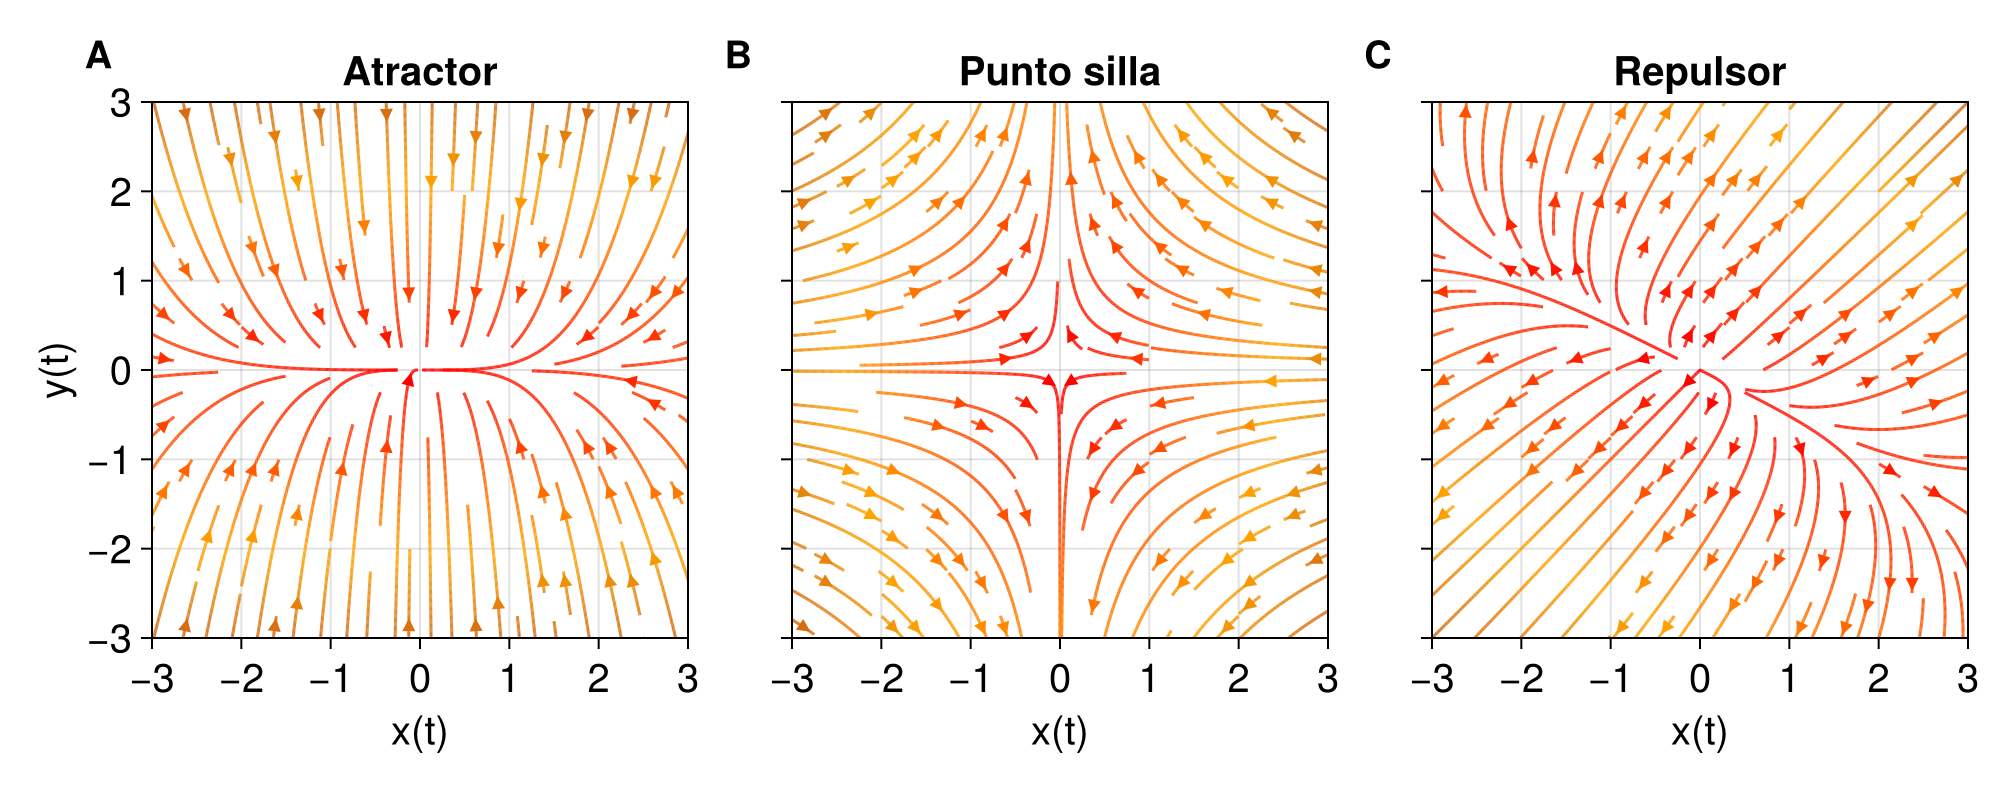
\includegraphics[scale=0.23]{../../Imagenes/Espacios fase reales}
		\caption{Espacios fase con eigenvalores reales. De izquierda a derecha se relacionan con las matrices del Ejemplo \ref{eg:EspaciosFreal}. La matriz $R_1$ corresponde con la gráfica de la izquierda, la matriz $R_2$ con la gráfica de en medio y la matriz $R_3$ con la gráfica de la derecha.}
		\label{fig:EFReales}
	\end{figure}
\end{ejemplo}

\begin{ejemplo}\label{eg:EspaciosFcomplejos}
	Para el caso de los espacios fase con eigenvalores complejos se proponen las siguientes matrices de coeficientes para $n=2$
	\begin{equation*}
		\begin{split}
			C_1=\begin{pmatrix}
				-2 & -3\\
				3 & -2 
			\end{pmatrix}
		\end{split},\qquad
		\begin{split}
			C_2=\begin{pmatrix}
				0 & 1\\
				-2 & 0 			
			\end{pmatrix}
		\end{split},\qquad
		\begin{split}
			C_3=\begin{pmatrix}
				0 & 2\\
				-3 & 2
			\end{pmatrix}
		\end{split}
	\end{equation*}
	Los eigenvalores para la matriz $C_1$ son $\lambda_{C_1}=-2\pm 3i$, nuevamente notamos que la parte real de sus eigenvalores son negativas lo que significa que todas las soluciones tenderán hacia el punto de equilibrio independientemente de sus condiciones iniciales; en la gráfica de la izquierda de la Figura (\ref{fig:EFComplejos}) se puede apreciar este comportamiento. Los eigenvalores de $C_2$ son respectivamente $\lambda_{C_2}=\pm 2i$, en este caso la parte real es igual a cero lo que significa que las soluciones van a estar oscilando para $t\to\infty$ sin llegar a converger a ningún punto, este tipo de comportamientos son ideales ya que en la naturaleza no se conoce alguna cosa que oscile de manera perpetua. Para los eigenvalores de $C_3$ se tienen los eigenvalores $\lambda_{C_3}=1\pm 5i$, en este caso las soluciones divergen (agregar más cosas...). Hablar con base de la solución general el caraceter oscilatorio de divergencia, convergencia y estacionario...
	\begin{figure}[h!]
		\centering
		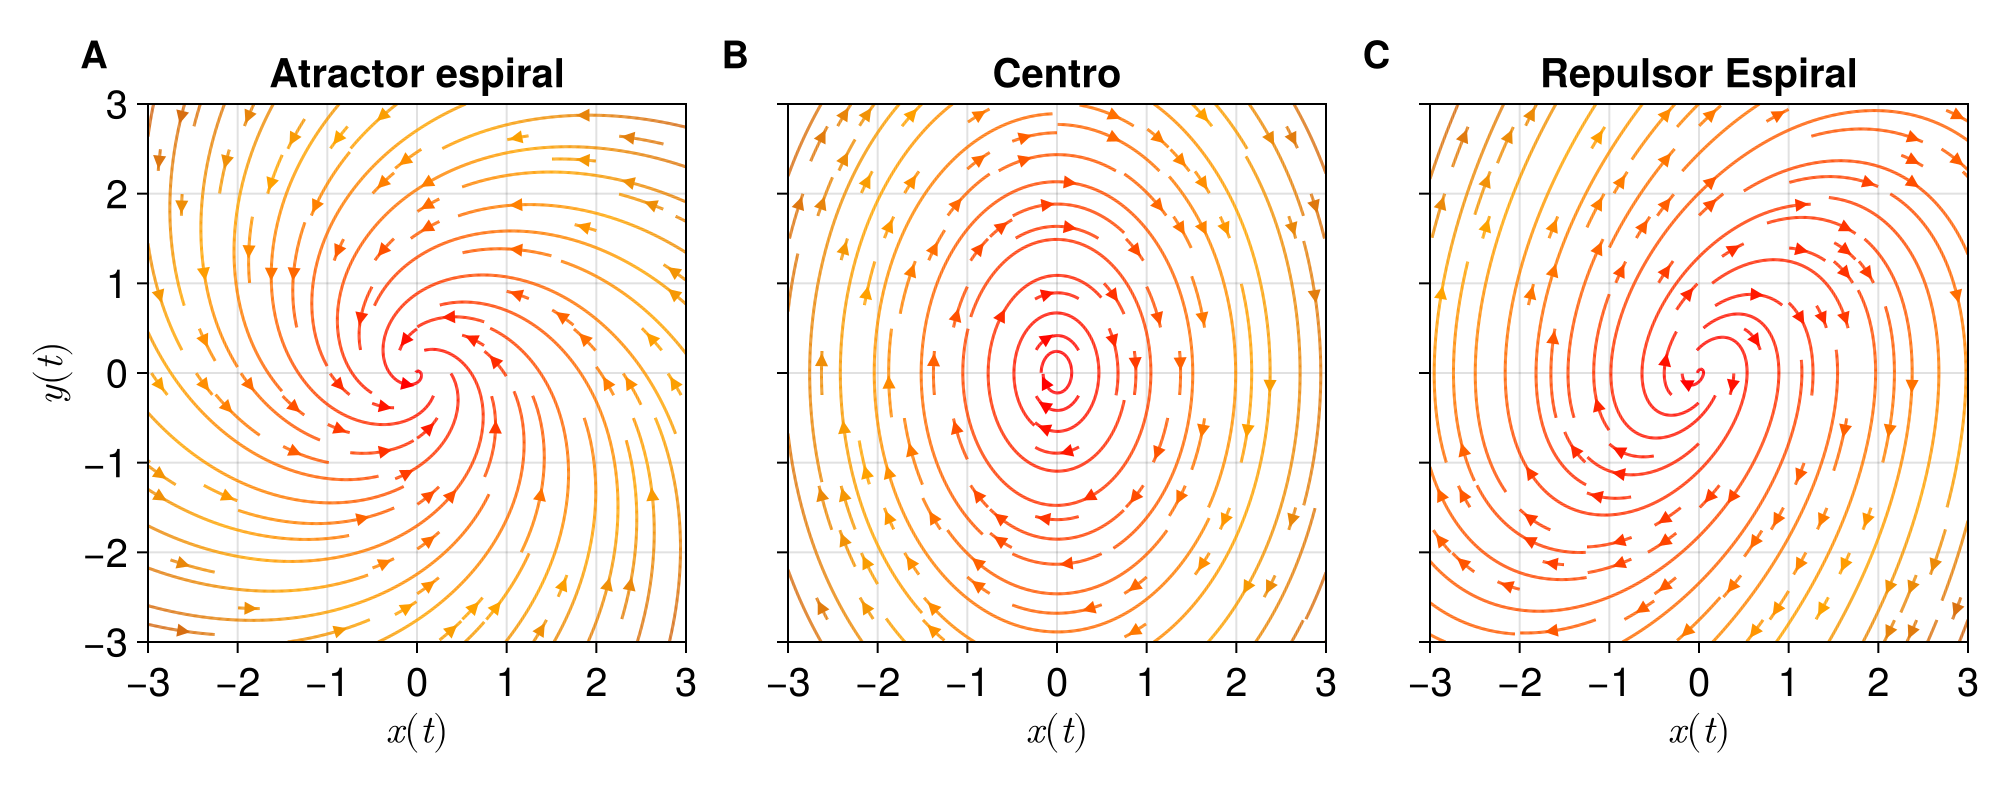
\includegraphics[scale=0.23]{../../Imagenes/Espacios fase complejos}
		\caption{Espacios fase con eigenvalores complejos. De izquierda a derecha se relacionan con las matrices del Ejemplo \ref{eg:EspaciosFcomplejos}. La matriz $C_1$ corresponde con la gráfica de la izquierda, la matriz $C_2$ con la gráfica de en medio y la matriz $C_3$ con la gráfica de la derecha.}
		\label{fig:EFComplejos}
	\end{figure}
\end{ejemplo}


\section{Sistemas no lineales}

\subsection{Modelo logístico}


%%la particularidad con los sistemas no lineales es el hecho de que no se pueden expresar como la suma de las soluciones del sistema, en otras palabras no cumplen el principio de superposición.